% $Header: /home/vedranm/bitbucket/beamer/solutions/generic-talks/generic-ornate-15min-45min.en.tex,v 90e850259b8b 2007/01/28 20:48:30 tantau $
\documentclass{beamer}
%\documentclass[handout]{beamer}
\usefonttheme[onlymath]{serif}
% This file is a solution template for:
\usepackage{algorithm}
\usepackage{algpseudocode}
% - Giving a talk on some subject.
% - The talk is between 15min and 45min long.
% - Style is ornate.



% Copyright 2004 by Till Tantau <tantau@users.sourceforge.net>.
%
% In principle, this file can be redistributed and/or modified under
% the terms of the GNU Public License, version 2.
%
% However, this file is supposed to be a template to be modified
% for your own needs. For this reason, if you use this file as a
% template and not specifically distribute it as part of a another
% package/program, I grant the extra permission to freely copy and
% modify this file as you see fit and even to delete this copyright
% notice. 

\mode<presentation>
{
  \usetheme{Warsaw}
  % or ...

  \setbeamercovered{transparent}
  % or whatever (possibly just delete it)
}
\setbeamertemplate{navigation symbols}{} 

\usepackage[english]{babel}
% or whatever

\usepackage[latin1]{inputenc}
% or whatever
\useoutertheme{default}

\usepackage{times}
\usepackage[T1]{fontenc}
% Or whatever. Note that the encoding and the font should match. If T1
% does not look nice, try deleting the line with the fontenc.
\newcommand{\beforeverb}{\footnotesize}
\newcommand{\afterverb}{\normalsize}

\title[Numerical Integration] % (optional, use only with long paper titles)
{Lecture 5}

\subtitle
{Numerical Integration} % (optional)

\author[Ying-Jer Kao] % (optional, use only with lots of authors)
{Ying-Jer Kao}
% - Use the \inst{?} command only if the authors have different
%   affiliation.

\institute[National Taiwan University] % (optional, but mostly needed)
{
  Department of Physics\\
 National Taiwan University
  }
% - Use the \inst command only if there are several affiliations.
% - Keep it simple, no one is interested in your street address.

\date[Numerical Analysis and Programming] % (optional)
{\today}

\subject{Talks}
% This is only inserted into the PDF information catalog. Can be left
% out. 



% If you have a file called "university-logo-filename.xxx", where xxx
% is a graphic format that can be processed by latex or pdflatex,
% resp., then you can add a logo as follows:

% \pgfdeclareimage[height=0.5cm]{university-logo}{university-logo-filename}
% \logo{\pgfuseimage{university-logo}}



% Delete this, if you do not want the table of contents to pop up at
% the beginning of each subsection:
%\AtBeginSubsection[]
%{
%  \begin{frame}<beamer>{Outline}
%    \tableofcontents[currentsection,currentsubsection]
%  \end{frame}
%}


% If you wish to uncover everything in a step-wise fashion, uncomment
% the following command: 

%\beamerdefaultoverlayspecification{<+->}


\begin{document}

\begin{frame}
  \titlepage
\end{frame}

\begin{frame}{Outline}
  \tableofcontents
  % You might wish to add the option [pausesections]
\end{frame}


% Since this a solution template for a generic talk, very little can
% be said about how it should be structured. However, the talk length
% of between 15min and 45min and the theme suggest that you stick to
% the following rules:  

% - Exactly two or three sections (other than the summary).
% - At *most* three subsections per section.
% - Talk about 30s to 2min per frame. So there should be between about
%   15 and 30 frames, all told.
\section[Introduction]{Introduction}
\begin{frame}{Introduction}
\begin{itemize}
\item Numerical integration, or \alert{quadrature}, approximates the definite integral 
\[
\int_a^b f(x)\; dx
\]
by 
\[
I=\sum_{i=0}^n A_i f(x_i)
\]
\item The \alert{nodal abscissas} $x_i$ and \alert{weights} $A_i$ depend on the particular rule used for the quadrature.
\item All rules of quadrature are derived from \alert{ polynomial interpolation} of the integrand.
\end{itemize}
\end{frame}

\begin{frame}{Quadrature}
\begin{itemize}
\item Methods of numerical integration can be divided into two groups: Newton-Cotes formulas and Gaussian quadrature. 
\item Newton-Cotes formulas are characterized by \alert{equally spaced abscissas} and include well-known methods such as the trapezoidal rule and Simpson's rule. 
\item They are most useful if $f(x)$ has already been computed at equal intervals or can be computed at low cost.
\item In Gaussian quadrature, the locations of the abscissas are chosen to yield the \alert{best possible accuracy}.
\item  It requires fewer evaluation of the integrand so It is useful if $f(x)$ is expensive to evaluate. 
\item It is capable of handling \alert{integrable singularities}, such as
\[
\int_0^1 \frac{g(x)}{\sqrt{1-x^2}} dx
\]
\end{itemize}
\end{frame}
\section[Newton-Cotes Formulas]{Newton-Cotes Formulas}
\begin{frame}{Newton-Cotes Formulas}

\begin{itemize}
\item Consider the definite integral: $
\int_a^b f(x) dx$.
\item Divide the range of integration $(a,b)$ into $n$ equal intervals of length $h=(b-a)/n$. 
\item Approximate $f(x)$ by a \alert{polynomial of degree $n$} that intersects all the all the nodes $x_0, x_1,\ldots, x_n$, in  Lagrange's form:
$P_n(x)=\sum_{i=0}^n f(x_i) l_i (x)$.
\item The integral is approximated by :
\end{itemize}
\begin{columns}
\begin{column}{0.6\textwidth}
\beforeverb
\[
I=\int_a^b P_n(x) dx =\sum_{i=0}^n \left[f(x_i) \int_a^b l_i (x) dx \right]=\sum_{i=0}^n A_i\, f(x_i)
\]
\afterverb
\end{column}
\begin{column}{0.4\textwidth}
\centerline{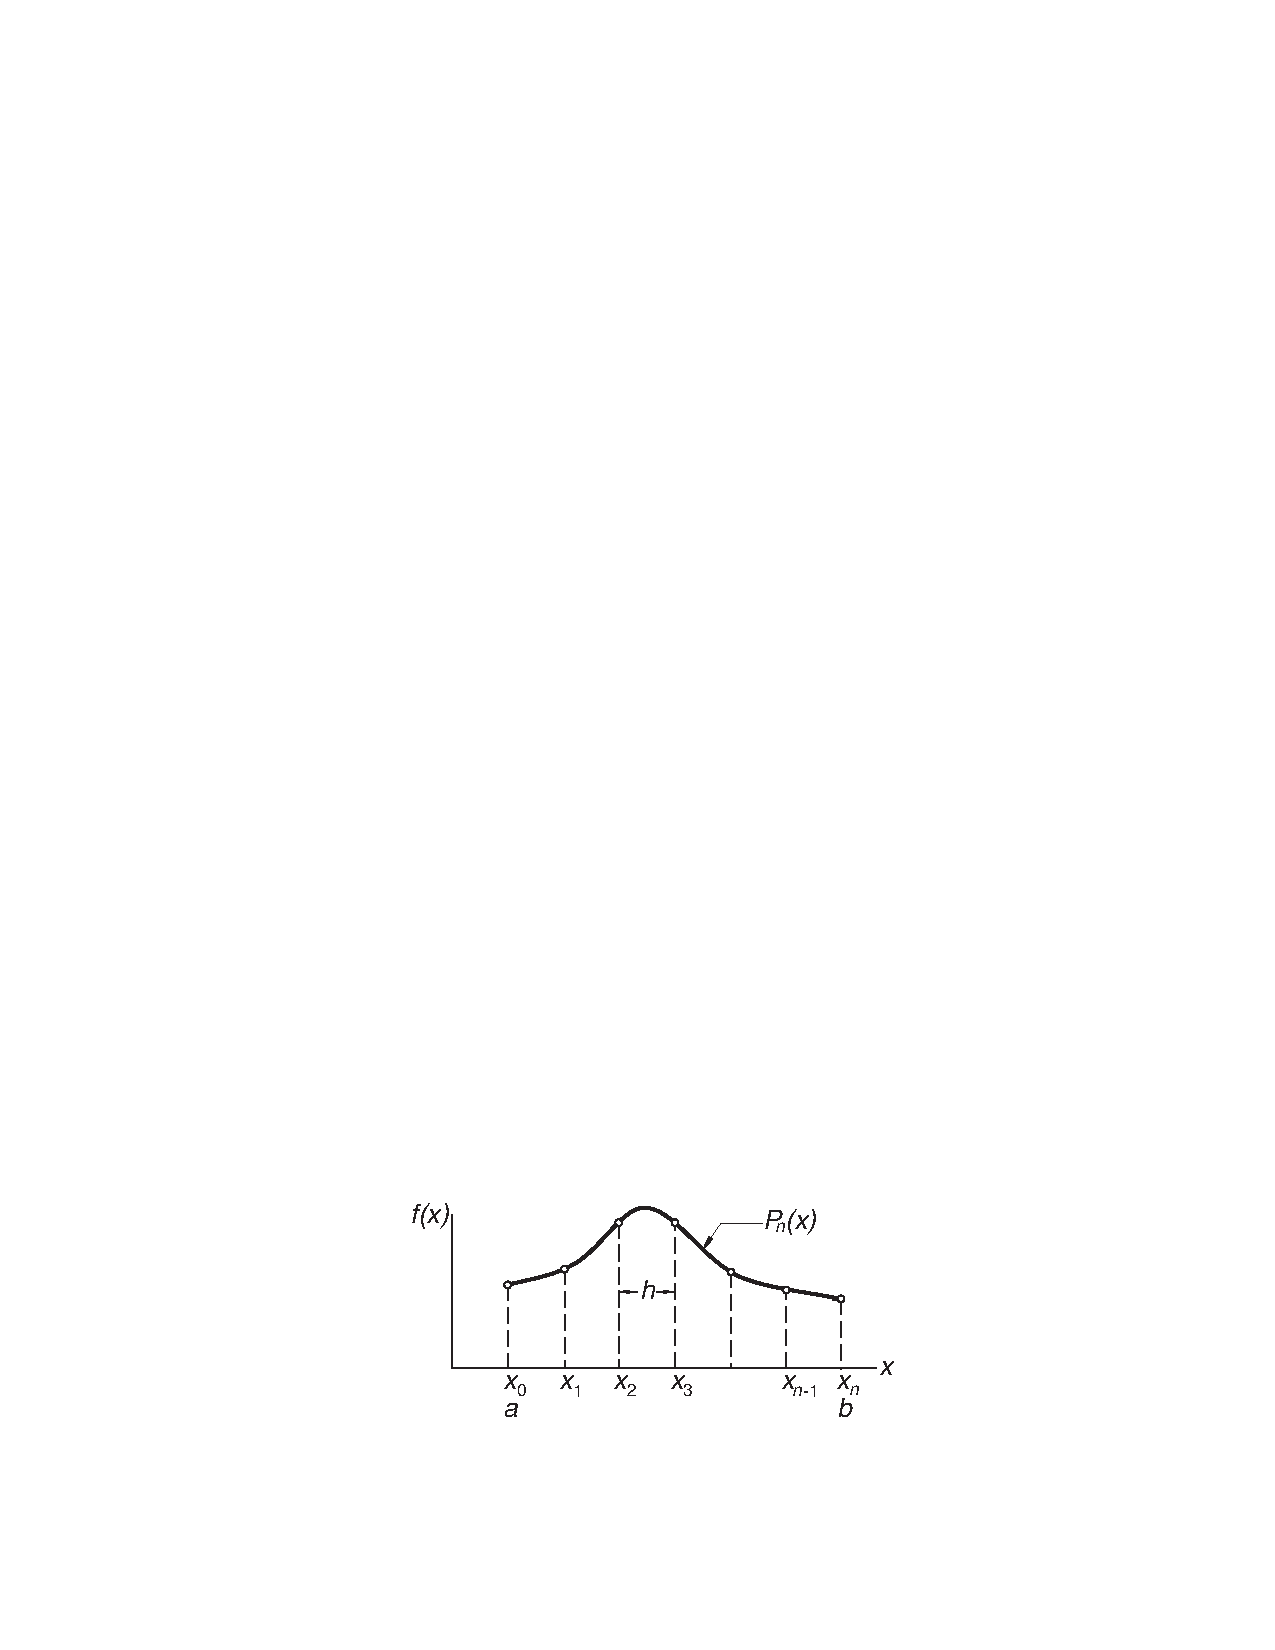
\includegraphics[width=\textwidth]{Lec12_Fig1}}
\end{column}
\end{columns}


\end{frame}


\subsection[Trapezoidal Rule]{Trapezoidal Rule}
\begin{frame}{Trapezoidal Rule}

\begin{itemize}
\item $n=1$, and $l_0=(x-x_1)/(x_0-x_1)=-(x-b)/h$,  $l_1=(x-x_0)/(x_1-x_0)=(x-a)/h$.
\item $A_0$ and $A_1$ are given by
\beforeverb
\begin{align*}
A_0&=\frac{1}{h} \int_a^b (x-b) dx =\frac{1}{2h}(b-a)^2=\frac{h}{2}\\
A_1&=\frac{1}{h} \int_a^b (x-a) dx =\frac{1}{2h}(b-a)^2=\frac{h}{2}
\end{align*}
\afterverb
\end{itemize}
\begin{columns}
\begin{column}{0.3\textwidth}
\centerline{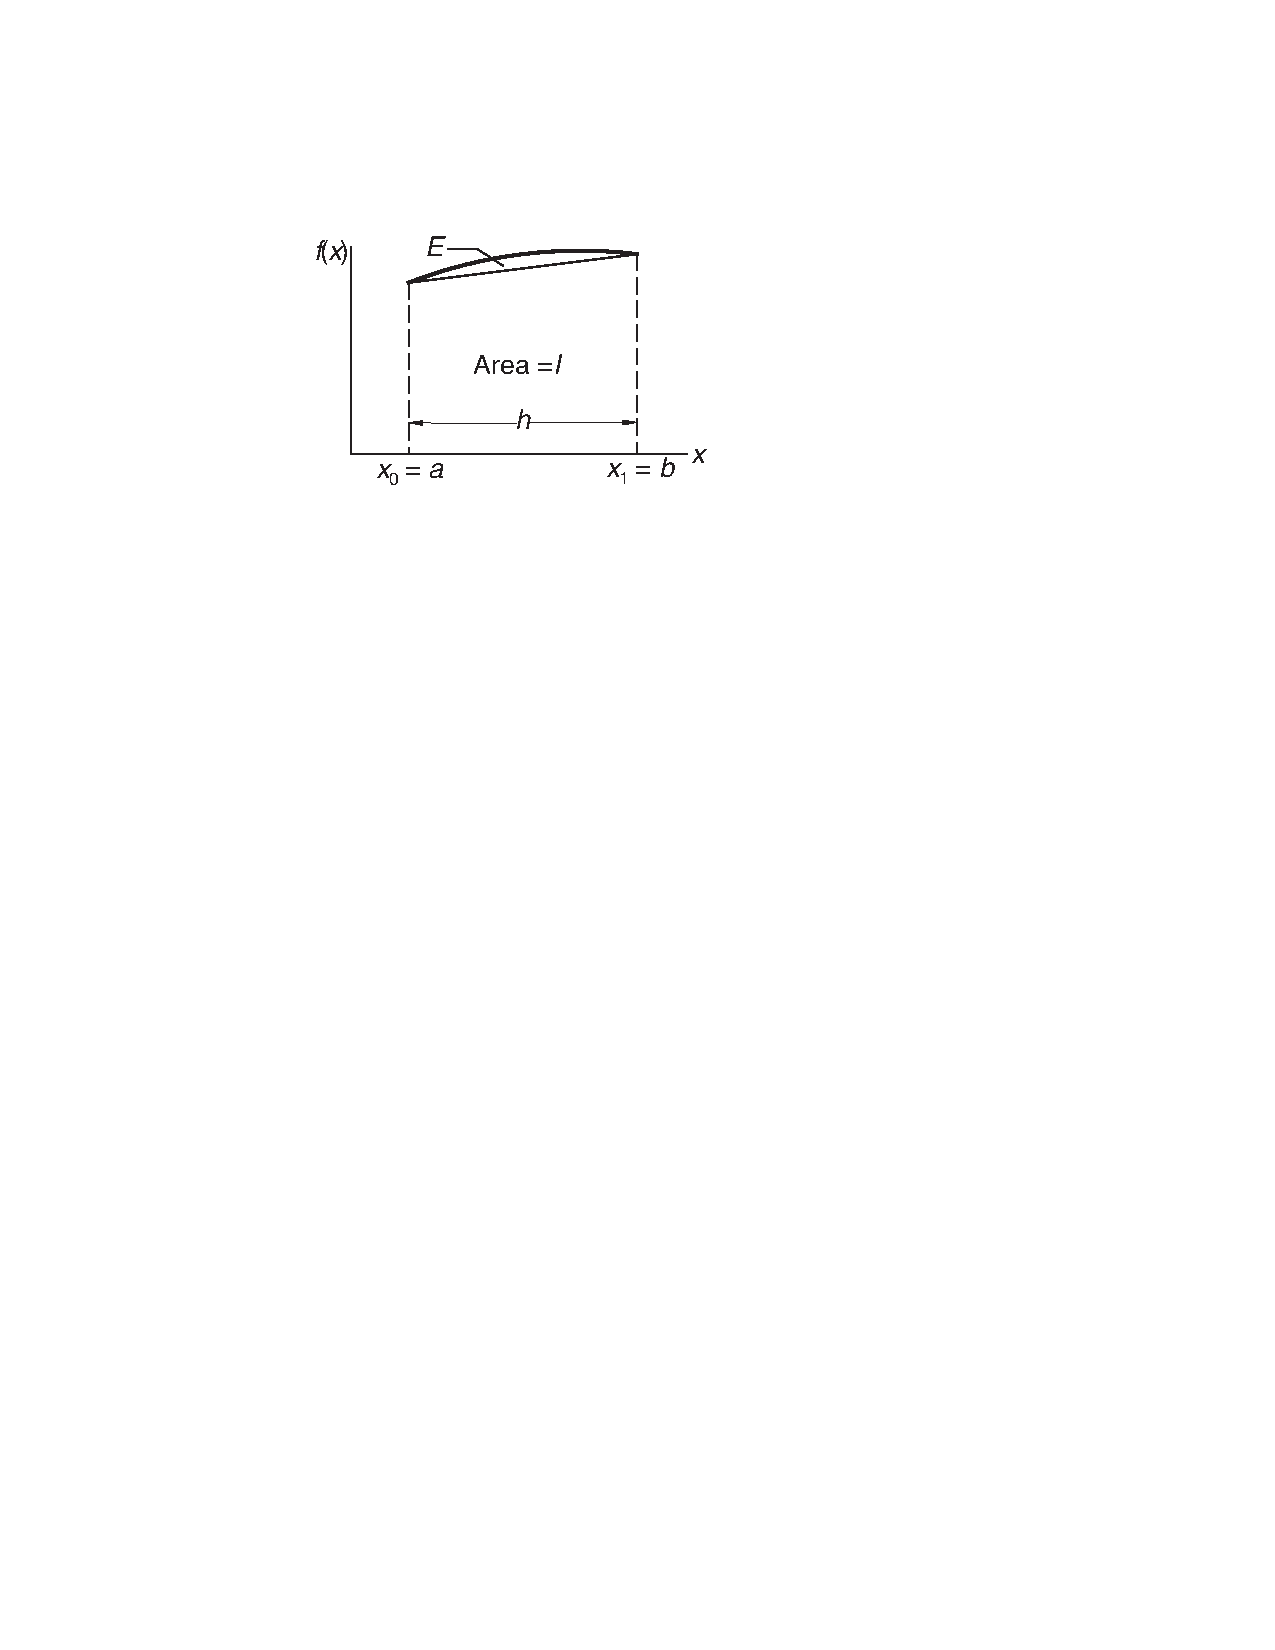
\includegraphics[width=\textwidth]{Lec12_Fig2}}
\end{column}

\begin{column}{0.7\textwidth}
\begin{itemize}
\item We have the \alert{trapezoidal rule},
\beforeverb
\[
I=[f(a)+f(b)]\frac{h}{2}
\]
\afterverb
\item Error in the trapezoidal rule
\beforeverb
\[
E=\frac{1}{2!}\int_a^b (x-x_0)(x-x_1) f''(\xi) dx =-\frac{h^3}{12}f''(\xi)
\]
\afterverb
\end{itemize}
\afterverb
\end{column}
\end{columns}
\end{frame}
\begin{frame}{Composite Trapezoidal Rule}
\begin{columns}
\begin{column}{0.4\textwidth}
\centerline{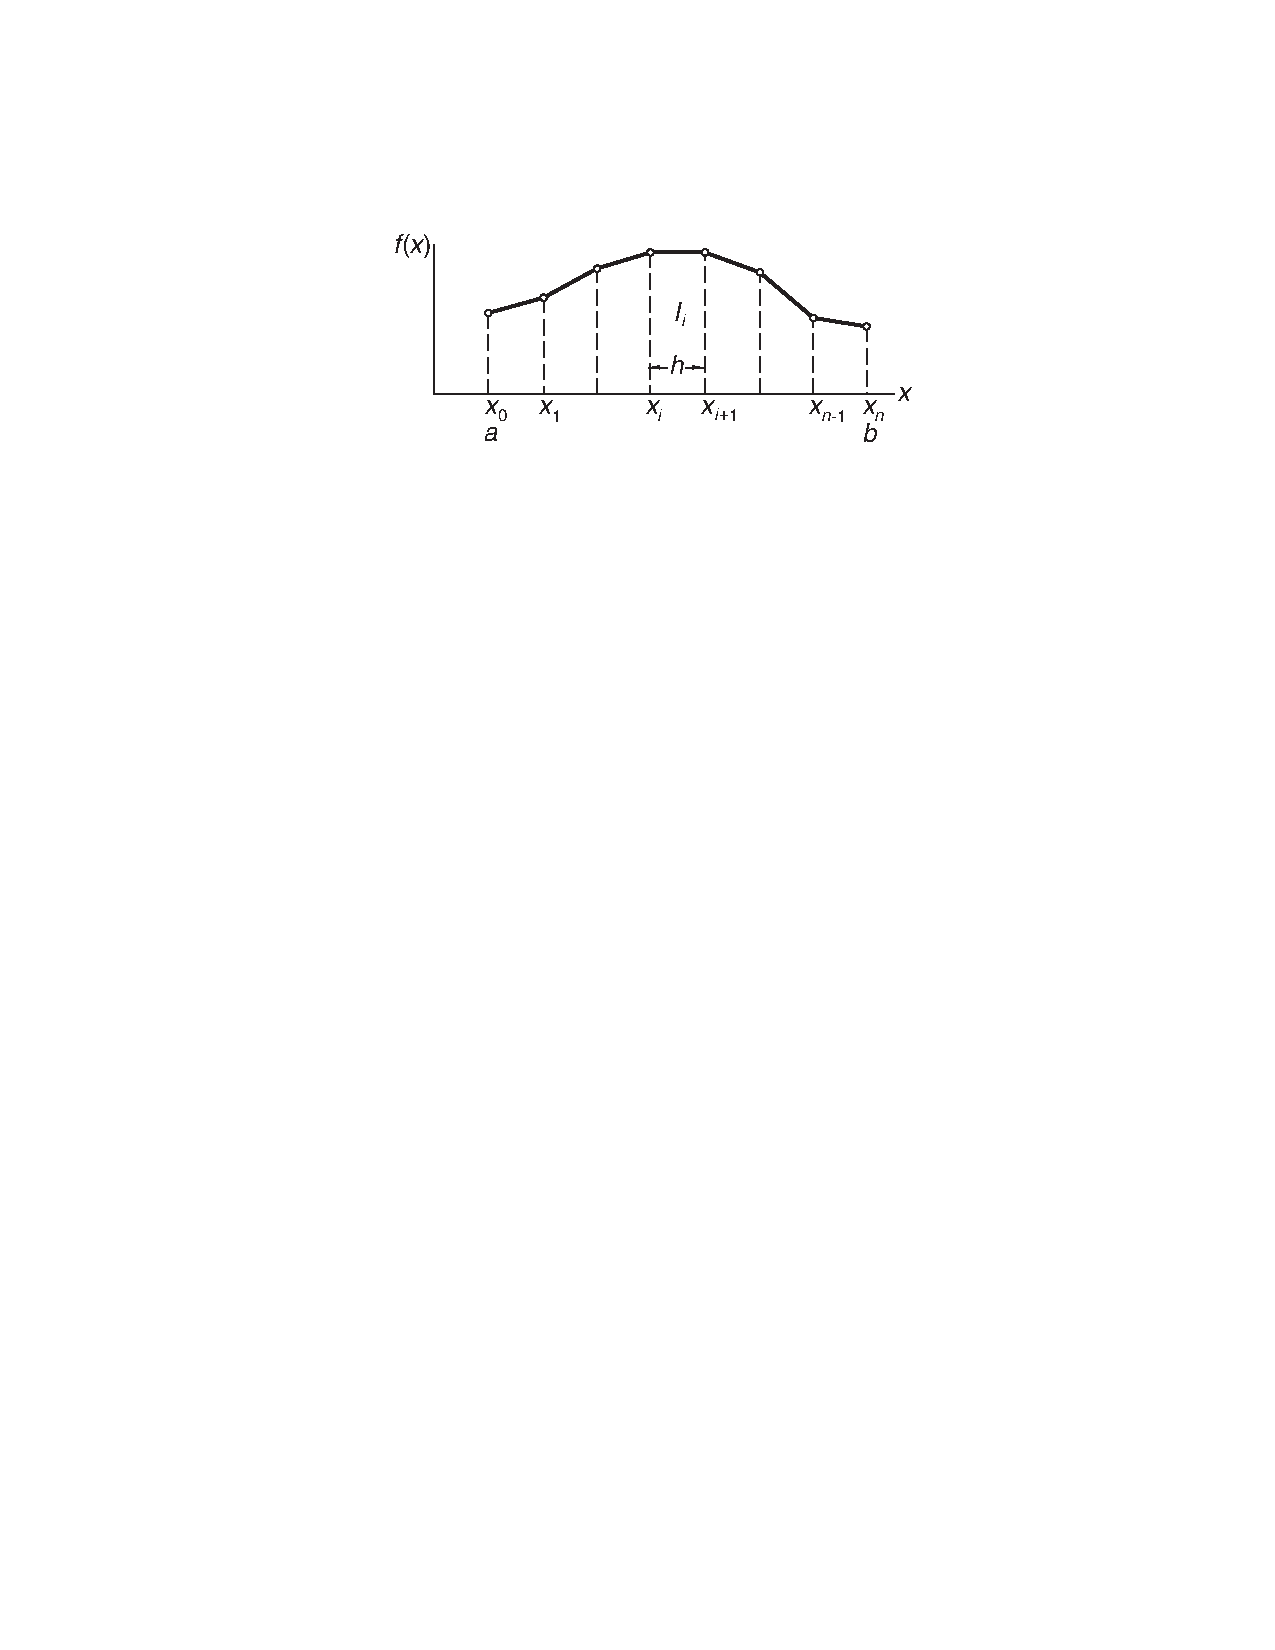
\includegraphics[width=\textwidth]{Lec12_Fig3}}
\end{column}
\begin{column}{0.7\textwidth}
\begin{itemize}
\item In practice, the trapezoidal rule is applied in a \alert{piecewise} fashion.
\item The interval $(a,b)$ is divided into $n$ subintervals, each with width $h$.
\end{itemize}
\afterverb
\end{column}

\end{columns}

\begin{itemize}
\item The approximate area of $i$th subinterval is given by the trapezoidal rule: 
$I_i=[f(x_i)+f(x_{i+1}) ]\frac{h}{2}$
\item The \alert{composite trapezoidal rule} gives the total area 
\beforeverb
\[
I=\sum_{i=0}^{n-1} I_i =[\,f(x_0)+2f(x_1)+2f(x_2)+\cdots+2f(x_{n-1}) +f(x_n)]\frac{h}{2}
\]
\afterverb
\item Truncation error 
\beforeverb
\[
E=\sum_{i=0}^{n-1}E_i=-\frac{h^3}{12}\sum_{i=0}^{n-1}f''(\xi_i)=-\frac{(b-a)h^2}{12}f''(\xi)=c_1h^2+c_2h^4 + \ldots
\]
\afterverb
\end{itemize}
\end{frame}
\begin{frame}{Recursive Trapezoidal Rule}
\begin{itemize}
\item $I_k$: integral evaluated with the composite trapezoidal rule using $2^{k}$ subintervals.
\item $H=b-a$: length of integration interval.
\item $k=0$: $I_0=[f(a)+f(b)]\frac{H}{2}$.
\item $k=1$:
\beforeverb
\[
I_1=\left[f(a)+2f\left(a+\frac{H}{2}\right)+f(b)\right]\frac{H}{4}=\frac{1}{2}I_0+f\left(a+\frac{H}{2}\right)\frac{H}{2}
\]
\afterverb
\item $k=2$:
\beforeverb
\begin{align*}
I_2&=\left[f(a)+2f\left(a+\frac{H}{4}\right)+2f\left(a+\frac{H}{2}\right)+2f\left(a+\frac{3H}{4}\right)+f(b)\right]\frac{H}{8}\\
&=\frac{1}{2}I_1+\left[f\left(a+\frac{H}{4}\right)+f\left(a+\frac{3H}{4}\right)\right]\frac{H}{2}
\end{align*}
\afterverb
\end{itemize}
\end{frame}
\begin{frame}{Recursive Trapezoidal Rule}
\begin{itemize}
\item For $k>0$, the \alert{recursive trapezoidal rule} is
\[
I_k=\frac{1}{2}I_{k-1}+\frac{H}{2^{k}}\sum_{i=1}^{2^{k-1}}f\left(a+\frac{(2i-1)H}{2^{k}}\right), \quad k=1,2,3,\ldots
\]
\afterverb
\item The summation contains only the \alert{new nodes} created when the number of subintervals is doubled. 
\item It is computationally as expensive as the original $I_k$ calculation using the composite trapezoidal rule.
\item Monitoring the difference between $I_{k-1}$ and  $I_k$ allows us to check the convergence.  
\end{itemize}

\end{frame}
\begin{frame}{Romberg Integration}
\begin{itemize}
\item Romberg integration combines the trapezoidal rule with Richardson extrapolation.
\item Let $R(i,0)=I_i$, the approximate integral computed by the recursive trapezoidal rule using $2^{i}$ subintervals.
\item The error of the trapezoidal rule is given as  $E=c_1h^2+c_2 h^4+\ldots,$ where $h=(b-a)/2^{i}$ is the width of a subinterval.
\item Romberg integration is based on the Richardson extrapolation
\beforeverb
\[
R(n,m)=R(n,m-1)+\frac{1}{4^m-1}[R(n,m-1)-R(n-1, m-1)], m\le1, n\le 1
\]
\afterverb
\end{itemize}
\end{frame}
\subsection[Simpson's Rules]{Simpson's Rules}
\begin{frame}{Simpson's Rules}
\begin{columns}
\begin{column}{0.4\textwidth}
\centerline{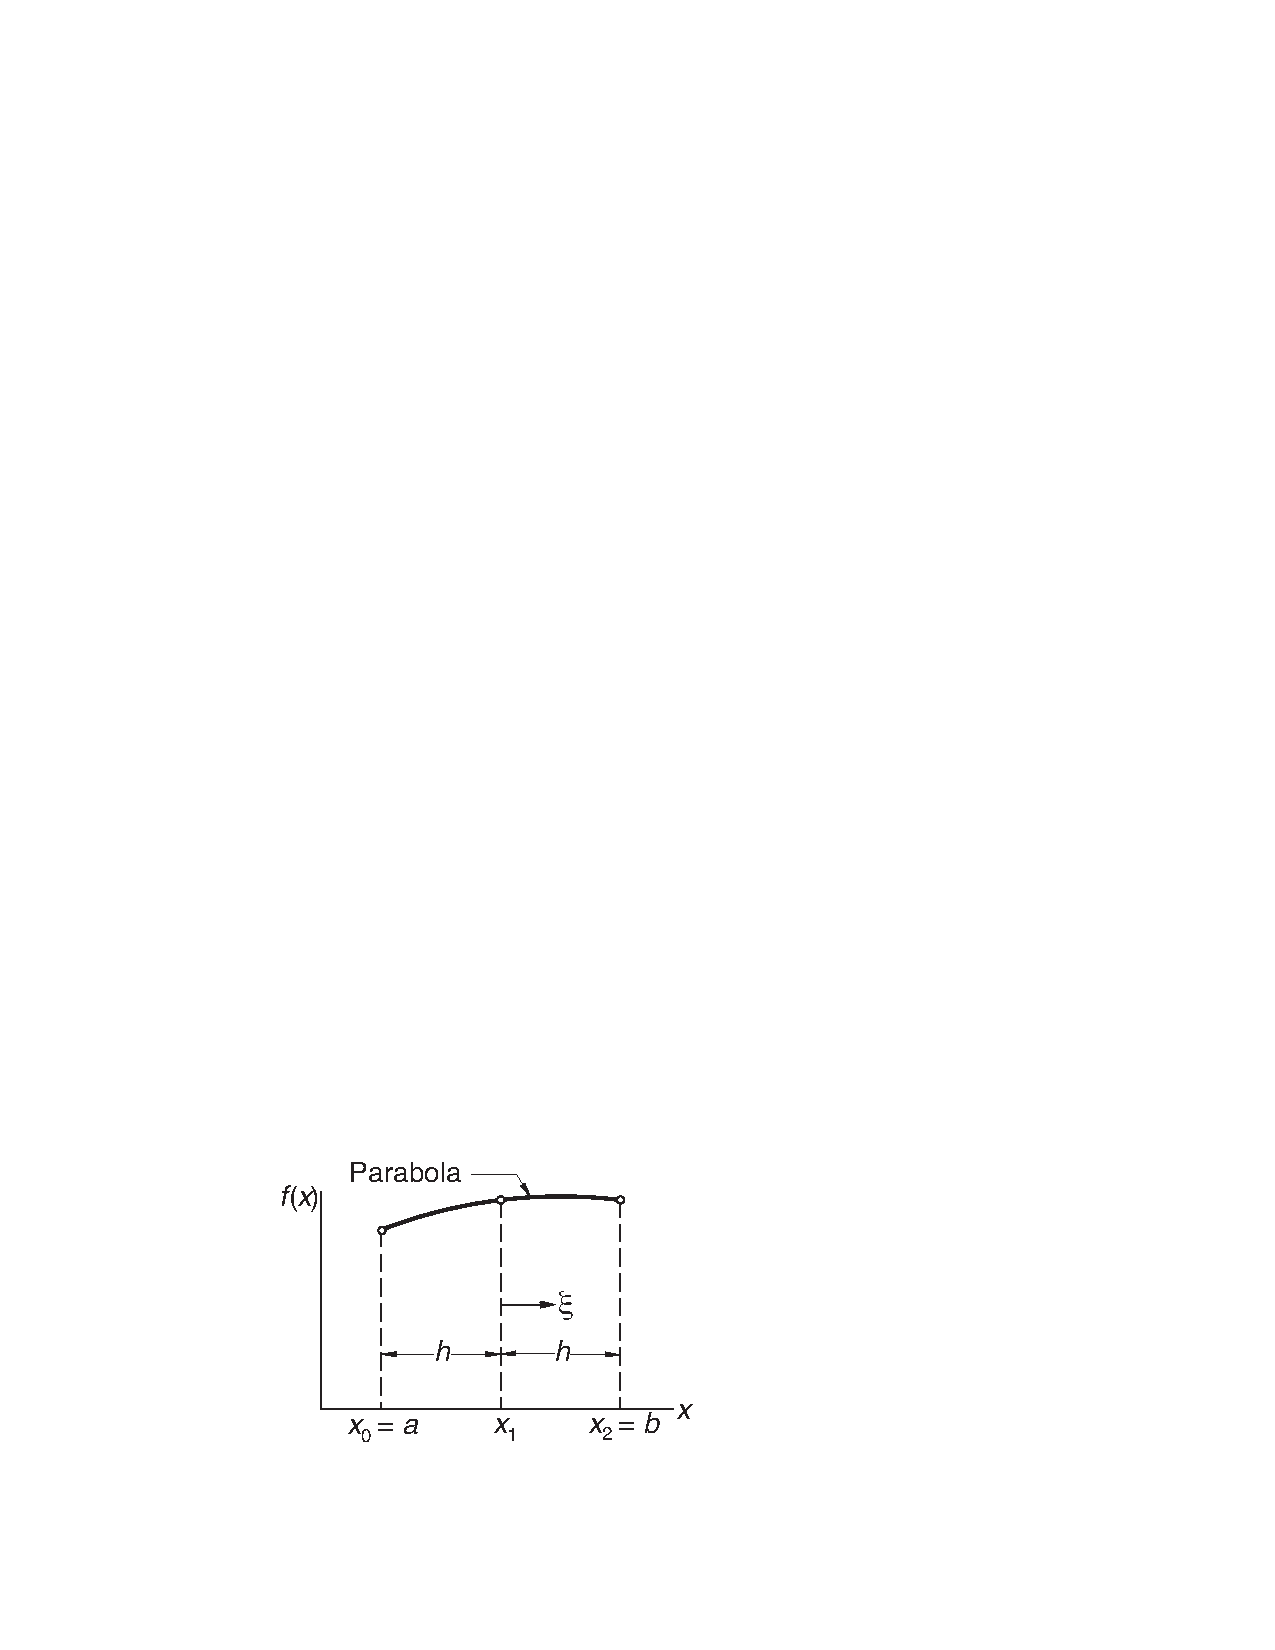
\includegraphics[width=\textwidth]{Lec12_Fig4}}
\end{column}
\begin{column}{0.7\textwidth}
\begin{itemize}
\item For $n=2$, using a parabolic interpolant through three adjacent nodes, we obtain the \alert{Simpson's 1/3 rule},
\end{itemize}
\beforeverb
\[
 I=\left[f(a)+4f\left(\frac{a+b}{2}\right)+f(b)\right]\frac{h}{3}
\]
\afterverb
\end{column}

\end{columns}
\begin{itemize}
\item The composite Simpson's 1/3 rule is obtained by dividing the integration range $(a, b)$ into $n$ ($n$ even) subintervals, and apply the Simpson's rule,
\begin{align*}
\int_a^b f(x) \, dx \approx I=&[f(x_0)+4f(x_1)+2f(x_2)+4f(x_3)+\ldots\\
&+2f(x_{n-2})+4f(x_{n-1})+f(x_n)]\frac{h}{3}
\end{align*}
\end{itemize}
\end{frame}
\begin{frame}{Error in Simpson's rule}
\begin{itemize}
\item The error in the composite Simpson's 1/3 rule is 
\[
E=\frac{(b-a)h^4}{180} f^{(4)}(\xi)
\]
\item Composite Simpson's 1/3 rule is \alert{exact} if $f(x)$ is a polynomial of degree 3 or less.
\item Number of subintervals $n$ has to be even. If $n$ is odd, we integrate over the first (or last) three subintervals with \alert{Simpson's 3/8 rule},
\[
I=[f(x_0)+3f(x_1)+3f(x_2)+f(x_3)]\frac{3h}{8}
\] 
\end{itemize}
\end{frame}
\section[Gaussian Quadrature]{Gaussian Quadrature}
\subsection[Gaussian Integration Formula]{Gaussian Integration Formula}
\begin{frame}{Gaussian Quadrature}
\begin{itemize}
\item Consider integrals of the form
\[
\int_a ^b \omega (x) f(x) dx
\]
where the weighting function $\omega(x)$ may contain integral singularities.
\item The integral can be approximated by 
\[
I=\sum_{i=0}^n A_i f(x_i).
\]
\item The nodes $x_i$ and weights $A_i$ are determined in Gaussian quadrature such that $I$ yields the exact integral if $f(x)$ is a polynomial of degree $\le 2n +1$.
\end{itemize}
\end{frame}
\begin{frame}{Gaussian Quadrature Theorem}
\begin{theorem}


Let $q$ be a nontrivial polynomial of degree $n+1$ such that
\[
\int_a^b x^k q(x) dx=0\quad (0\le k\le n)
\]
Let $x_0, x_1, \ldots, x_n$ be the zeros of $q$. With these $x_i$'s as nodes, 
\[
\int_a^b f(x) \omega(x) dx \approx \sum_{i=0}^n A_i f(x_i) \quad\mbox{where} \quad A_i=\int_a^b l_i(x)\omega(x)  dx 
\]
will be exact for all polynomials of degree at most $2n+1$, and the nodes lie in the open interval $(a,b)$.
\end{theorem}
\end{frame}
\begin{frame}{Gaussian Integration Formula}
\begin{itemize}
\item If $f(x)=P_m(x)$ is a polynomial of degree $m$, $x_i$ and $A_i$ are determined such that,
\[
\int_a ^b \omega(x) P_m(x)\; dx =\sum_{i=0}^n A_i P_m(x_i), \quad m\le 2n+1
\]
\item Assume $P_0(x)=1, P_1(x)=x, P_2(x)=x^2, \ldots, P_{2n+1}(x)=x^{2n+1}$, and we obtain $2n+2$ equations,
\[
\int_a ^b \omega(x) x^j \; dx =\sum_{i=0}^n A_i x^j_i, \quad (j=0, 1, \ldots, 2n+1)
\]
which can be solved for the $2n+2$ unknowns $A_i, x_i$.
 
\end{itemize}
\end{frame}
\begin{frame}{Gaussian Quadrature: Example}
\begin{itemize}
\item Let $\omega(x)=e^{-x}, a=0, b=\infty$, and $n=1$. 
\item Equations for $x_0, x_1, A_0, A_1$ are
\beforeverb
\begin{align*}
\int_0^\infty e^{-x} dx&=A_0+A_1 &  x_0&= 2-\sqrt{2}  \\
\int_0^\infty e^{-x} x dx&=A_0 x_0 +A_1 x_1 &\Rightarrow \quad x_1&=2+\sqrt{2}\\
\int_0^\infty e^{-x} x^2 dx&=A_0 x_0^2+A_1 x_1^2 & A_0&=\frac{\sqrt{2}+1}{2\sqrt{2}}\\
\int_0^\infty e^{-x} x^3 dx&=A_0 x_0^3+A_1 x_1^3  &A_1&=\frac{\sqrt{2}-1}{2\sqrt{2}} 
\end{align*}
\afterverb
\item The integration formula is 
\beforeverb
\[
\int_0^\infty e^{-x} f(x) \approx \frac{1}{2\sqrt{2}} \left[(\sqrt{2}+1)f(2-\sqrt{2})+(\sqrt{2}-1)f(2+\sqrt{2})\right]
\]
\afterverb
\end{itemize}
\end{frame}
\begin{frame}{Classical Gaussian Quadratures}
\begin{itemize}
\item Nodal abscissas and weights in Gaussian integration formulas can be obtained using \alert{orthogonal polynomials}. The nodes are just the zeros of the polynomial.
\item Commonly used polynomials are Legendre, Chebyshev, Laguerre, and Hermite polynomials.
\item For Legendre polynomials, $P_n(x)$, with the $n$th polynomial normalized to give $P_n(1)=1$, the $i$th Gaussian node is the $i$th zero of $P_n(x)$, and the weights $A_i$ are given by
\beforeverb
\[
A_i=\frac{2}{(1-x_i^2)[P'_{n+1}(x_i)]^2}
\]
\afterverb
\end{itemize}
\end{frame}
\subsection[Gauss-Legendre Quadrature]{Gauss-Legendre Quadrature}
\begin{frame}{Gauss-Legendre Quadrature}
\begin{itemize}
\item A commonly used quadrature is the Gauss-Legendre integration formula, 
\[
\int_{-1}^1 f(x) dx = \sum_{i=0}^n A_i f(\xi_i)
\]
\item The nodes $\xi_i$ are arranged symmetrically about $\xi=0$, and the weights associated with a
symmetric pair of nodes are equal. 
\item For $n=1$, $\xi_0=-\xi_1$ and $A_0=A_1$.
\item The truncation error is 
\[
E=\frac{2^{2n+3}[(n+1)!]^4}{(2n+3)[(2n+2)!]^3}\,f^{2n+2}(c), \quad -1<c<1
\]
\end{itemize}
\end{frame}
\begin{frame}{Change of Interval}
\begin{itemize}
\item To apply the Gauss-Legendre quadrature, we need to change the integration interval from $(a,b)$ to $(-1,1)$,
\begin{align*}
\int_a^b f(x) dx &=\frac{b-a}{2}\int_{-1}^1 f\left(\frac{b-a}{2}x+\frac{b+a}{2}\right)\,dx	\\
&\approx \frac{b-a}{2}\sum_{i=1}^n A_i  f\left(\frac{b-a}{2}x+\frac{b+a}{2}\right) 
\end{align*}
\end{itemize}
\end{frame}
\begin{frame}{Gauss-Legendre Quadrature Nodes and Weights}

%\begin{columns}
%\begin{column}{0.5\textwidth}
\begin{itemize}
\item The nodes and weights of Gauss-Legendre integration formula for $n=1, 2, 3, 4 $ are listed below.
\end{itemize}
%\beforeverb
\begin{center}
\begin{tabular}{|l|l|l|}
\hline
$n$& Nodes $\xi_i$ & Weights $A_i$ \\
\hline
1 & $\pm\sqrt{1/3}$ & 1\\
\hline
2 & $\pm\sqrt{3/5}$ & $5/9$ \\
 & 0 & $8/9$ \\
\hline
3 & $\pm\sqrt{1/7(3-4\sqrt{3/10})}$ & $\frac{18+\sqrt{30}}{36}$ \\
 & $\pm\sqrt{1/7(3+4\sqrt{3/10})}$ & $\frac{18-\sqrt{30}}{36}$ \\\hline
%\end{tabular}
%\end{center}
%\end{column}
%\begin{column}{0.5\textwidth}
%\begin{center}
%\begin{tabular}{|l|l|l|}
%\hline 
%$n$ & Nodes $\xi_i$ & Weights $A_i$ \\
%\hline 
4 & $\pm1/3\sqrt{5-2\sqrt{10/7}}$ & $\frac{322+13\sqrt{70}}{900}$ \\
& $\pm1/3 \sqrt{5+2\sqrt{10/7}}$ & $\frac{322-13\sqrt{70}}{900}$ \\
&0 & $128/225$\\ \hline 

\end{tabular}
\end{center}
%\end{column}
%\end{columns}
\afterverb
\end{frame}
\begin{frame}{Classical Gaussian Quadrature}
\begin{itemize}
\item Some of the classical Gaussian quadrature formulas for the integral
\[
\int_a^b \omega(x) f(x) dx
\]
are:
\end{itemize}
\begin{center}
\begin{tabular}{|l|l|l|}
\hline
 $\omega(x)$ & interval & $x_i$ are roots of \\
\hline
$1$ & $(-1,1)$ & $P_n(x)$, Legendre \\
$e^{-x}$ & $[0,\infty)$& $L_n(x)$, Leguerre \\
$e^{-x^2}$ & $(-\infty,\infty)$& $H_n(x)$, Hermite \\
$1/\sqrt{1-x^2}$ & $(-1,1)$ & $T_n(x)$, Chebychev  (1st kind)\\
$\sqrt{1-x^2}$ & $(-1,1)$ & $U_n(x)$, Chebychev   (2nd kind)	\\
\hline	
\end{tabular}
\end{center}

\end{frame}
\begin{frame}{Integrals with Singularities}
\begin{itemize}
\item An important case where Gaussian formulas have an advantage occurs in integrating a
function that is \alert{infinite at one end of the interval}.
\item The nodes in Gaussian quadrature are always \alert{interior points} of the interval.
\item For example,
%\beforeverb
%\[
$\int_0^1\frac{\sin x}{x} dx$ 
%\]
%\afterverb
can be evaluated by the substitution $y\leftarrow \sin x/x$ with a Gaussian formula since the value $x=0$ is not required.
\item More difficult integrals such as 
%\beforeverb
%\[
$\int_0^1 \frac{\sqrt[3]{x^2-1}}{\sqrt{\sin(e^x-1)}} dx$
%\]
%\afterverb
can be evaluated directly with a Gaussian formula despite the singularity at $x=0$.
\end{itemize}
\end{frame}

\begin{frame}{Multi-dimensional Integration}
\begin{itemize}
  \item For simlicity, consider the trapezoid rule for the interval $[0,1]$, using $n$ subintervals with step size $h=1/n$.
  $$
\int_0^1 f(x) d x \approx \frac{1}{2 h}\left[f(0)+2 \sum_{i=1}^{n-1} f\left(\frac{i}{n}\right)+f(1)\right]\approx \sum_{i=0}^n C_i f\left(\frac{i}{n}\right)
$$
\item 
The error is $ \mathcal{O}\left(h^2\right)=\mathcal{O}\left(n^{-2}\right)  $
for functions having a continuous second derivative. 
\end{itemize}
\end{frame}
\begin{frame}{Multi-dimensional Integration}
  \begin{itemize}
    \item A two-dimensional integration over the unit square, 
    $$
\begin{aligned}
\int_0^1 \int_0^1 f(x, y) d x d y & \approx \int_0^1 \sum_{\alpha_1=0}^n C_{\alpha_1} f\left(\frac{\alpha_1}{n}, y\right) d y \\
& =\sum_{\alpha_1=0}^n C_{\alpha_1} \int_0^1 f\left(\frac{\alpha_1}{n}, y\right) d y \\
& \approx \sum_{\alpha_1=0}^n C_{\alpha_1} \sum_{\alpha_2=0}^n C_{\alpha_2} f\left(\frac{\alpha_1}{n}, \frac{\alpha_2}{n}\right) \\
& =\sum_{\alpha_1=0}^n \sum_{\alpha_2=0}^n C_{\alpha_1} C_{\alpha_2} f\left(\frac{\alpha_1}{n}, \frac{\alpha_2}{n}\right)
\end{aligned}
$$
\item The error is  $\mathcal{O}(h^2)=\mathcal{O}(n^{-2})=\mathcal{O}\left(N^{-4}\right)  $ for functions having a continuous second derivative, where $N=n^2$.
  \end{itemize}
\end{frame}

\begin{frame}{Multi-dimensional Integration}
  \begin{itemize}
    \item A $k$-dimensional integration over the 
$k$-dimensional cube $[0,1]^k \equiv[0,1] \times[0,1] \times \cdots \times[0,1]$,
$$
\int_{[0,1\}^{\prime}} f(x) d x \approx \sum_{\alpha_1=0}^n \sum_{\alpha_1=0}^n \cdots \sum_{\alpha_k=0}^n C_{\alpha_1} C_{\alpha_2} \cdots C_{\alpha_1} f\left(\frac{\alpha_1}{n}, \frac{\alpha_2}{n}, \ldots, \frac{\alpha_k}{n}\right)
$$
\item The error is  $\mathcal{O}(h^2)=\mathcal{O}(n^{-2})=\mathcal{O}((n^{k})^{-2/k})=\mathcal{O}\left(N^{-2/k}\right)  $.
\item The quality of the numerical approximation of the integral declines as $k$ increases. 
\item If a constant order of accuracy is to be retained while the number of variables, $k$, goes up, the number of nodes must go up like $n^k$. 
\item The Monte Carlo method for numerical integration becomes more attractive for high-dimensional integration.
  \end{itemize}
\end{frame}
\end{document}


